\chapter{Implementacija i korisničko sučelje}
		
		
		\section{Korištene tehnologije i alati}
		Pisana komunikacija u timu odvijala se putem aplikacije WhatsApp\footnote{https://www.whatsapp.com/}, a sastanci putem Google Meeta\footnote{https://meet.google.com/} i Discorda\footnote{https://discord.com/}. WhatsApp je besplatna mobilna aplikacija koja služi za razmjenu poruka, fotografija i videozapisa putem mobilnog interneta pametnim telefonom. Google Meet je usluga videokomunikacije koju je razvio Google, dok je Discord VoIP aplikacija koja omogućava komunikaciju glasom, videom i tekstom.
		
		UML dijagrami napravljeni su alatom Visual Paradigm Online\footnote{https://online.visual-paradigm.com/}. Visual Paradigm Online je online alat za crtanje dijagrama i njihovu pohranu u web-pregledniku koji omogućava istovremeni rad više korisnika u stvarnom vremenu. Dijagrame možemo preuzeti u raznim formatima (.png, .jpeg, .pdf i dr.).
		
		Za vizualizaciju stranice korištena je Figma\footnote{https://www.figma.com/}, besplatan alat za UI i UX dizajn, uređivanje i izradu	prototipova te generiranje koda dostupan na webu ili u obliku desktop aplikacije.
		
		Izvornim kodom upravljano je sustavom Git\footnote{https://git-scm.com/}. Git je distribuirani sustav za upravljanje različitim	verzijama podataka (programskog koda, teksta i dr.). Sastoji se od udaljenog repozitorija koji se nalazi na nekoj Git platformi u oblaku i od lokalnih kopija tog repozitorija na računalima korisnika koji rade na projektu. Udaljeni repozitorij ovog projekta dostupan je na web platformi Gitlab\footnote{https://about.gitlab.com/}.
		
		Kao razvojno okruženje korišten je Visual Studio Code\footnote{https://code.visualstudio.com/}. Visual Studio Code
		je uređivač izvornog koda koji je razvio Microsoft za Linux, Windows i Mac OS platforme. Uključuje podršku za uklanjanje pogrešaka, isticanje sintakse, inteligentno dovršavanje koda, isječke, refaktoriranje koda i ugrađeni Git.
		
		Osim VSCode-a, koristili smo i JetBrains WebStorm\footnote{https://www.jetbrains.com/webstorm/} i JetBrains DataGrip\footnote{https://www.jetbrains.com/datagrip/}. WebStorm je integrirana razvojna okolina za JavaScript i povezane tehnologije, a DataGrip detektira moguće \textit{buggove} u kodu i predlaže najbolje opcije za njihovo ispravljanje.
		
		Cijeli sustav pisan je jezikom TypeScript\footnote{https://www.typescriptlang.org/} koji je proširenje jezika JavaScript(JavaScript s tipovima), skriptnog programskog jezika koji omogućava interakciju korisnika s web-stranicom.
		
		Za frontend smo koristili React\footnote{https://reactjs.org/} i Chakra UI\footnote{https://chakra-ui.com/}. React je knjižnica koja služi za izgradnju korisničkog sučelja ili UI komponenti, a Chakra je jednostavna modularna bibloteka komponenata	u kojoj se nalaze blokovi potrebni za izgradnju React aplikacija.
		
		 PostgreSQL\footnote{https://www.postgresql.org/} baza podataka spremljena je na serveru. PostgreSQL je besplatni i relacijski sustav upravljanja bazom podataka otvorenog koda dizajniran za upravljanje nizom radnih opterećenja, od pojedinačnih strojeva do skladišta podataka ili web-usluga s mnogim istovremenim korisnicima. Naš server nalazi se na Vultr VPS\footnote{https://vultr.com} serveru.
		
			\eject 
		
	
		\section{Ispitivanje programskog rješenja}
			
			\subsection{Ispitivanje komponenti}
			
			\noindent \underbar{\textbf{Testni Slučaj 1}}
			\begin{lstlisting}
				const mocks = [
					{
					  request: { query: me },
					  result: {
						data: {
						  me: null,
						},
					  },
					},
				  ];
				  
				  describe("Actual", () => {
					it("renders a heading", () => {
					  render(
						<MockedProvider mocks={mocks} addTypename={false}>
						  <ActualEarthquakesPage />
						</MockedProvider>
					  );
				  
					  const heading = screen.getByText("Loading...");
					  expect(heading).toBeInTheDocument();
					});
				  });
			\end{lstlisting}

			\noindent \underbar{\textbf{Testni Slučaj 2}}
			\begin{lstlisting}
				const mocks = [
					{
					  request: { query: me },
					  result: {
						data: {
						  me: null,
						},
					  },
					},
				  ];
				  
				  const earthquakesMock = {
					request: { query: earthquakes, variables: { archived: true } },
					result: {
					  data: {
						earthquakes: [],
					  },
					},
				  };
				  
				  describe("Archived", () => {
					it("renders a loading", () => {
					  render(
						<MockedProvider mocks={mocks} addTypename={false}>
						  <ArchivedEarthquakesPage />
						</MockedProvider>
					  );
				  
					  const heading = screen.getByText("Loading...");
					  expect(heading).toBeInTheDocument();
					});
				  });
			\end{lstlisting}

			\bigskip

			\noindent \underbar{\textbf{Testni Slučaj 3}}
			\begin{lstlisting}
				const mocks = [
					{
					  request: { query: me },
					  result: {
						data: {
						  me: null,
						},
					  },
					},
				  ];
				  
				  describe("Home", () => {
					it("renders a heading", () => {
					  render(
						<MockedProvider mocks={mocks} addTypename={false}>
						  <Navigation />
						</MockedProvider>
					  );
				  
					  const heading = screen.getByRole("heading", {
						name: /TECTONIC HR/i,
					  });
				  
					  expect(heading).toBeInTheDocument();
					});
				  });
			\end{lstlisting}

			\noindent \underbar{\textbf{Testni Slučajevi 4, 5, 6}}
			\begin{lstlisting}
				describe("Intensity generation", () => {
					it("Expect to check simple", () => {
					  const data = ["1", "5", "5", "5", "3"];
					  expect(calcIntensity(data)).toBe(5);
					});
				  
					it("Expect to more stuff simple", () => {
					  const data = ["1", "<=3", ">=8", "7", "6", "<=4", "5", "5", "5", "3"];
					  expect(calcIntensity(data)).toBe(8);
					});
				  
					it("Expect to or simple", () => {
					  const data = ["1", "2|3"];
					  expect(calcIntensity(data)).toBe(3);
					});
				  });
			\end{lstlisting}
			
			\subsection{Ispitivanje sustava}
			 
			 \noindent \underbar{\textbf{Testni Slučaj 1: Prijava s ispravnim podacima}}
			 \begin{packed_item}

				 \item \textbf{Ulaz:}

				 \item[] \begin{packed_enum}
					\item email: "foo@bar.com"
					\item password: "foobar123"
				\end{packed_enum}

				  \item \textbf{Očekivani izlaz:}

				 \item[] \begin{packed_enum}
					\item prijava u sustav
					\item preusmjerenje na početnu stranicu
				\end{packed_enum}
				 
				\item \textbf{Rezultat:}

				\item[] \begin{packed_enum}
					\item prijava u sustav
					\item preusmjerenje na početnu stranicu
			   \end{packed_enum}

			 \end{packed_item}
			 \begin{lstlisting}
				@Test()
				public void loginTestGoodCredentials() {
					System.setProperty("webdriver.chrome.driver", "C:\\Program Files\\chromedriver\\chromedriver.exe");
					WebDriver driver = new ChromeDriver();
					driver.manage().timeouts().implicitlyWait(10, TimeUnit.SECONDS);
					// posjeti web stranicu
					driver.get("https://tectonichr.tk/");

					// otvori izbornik s gumbom za prijavu
					WebElement element = driver.findElement(By.id("menu-button-2"));
					element.click();

					// otvori stranicu za prijavu
					element = driver.findElement(By.id("menu-list-2"));
					element.click();

					// unesi email
					element = driver.findElement(By.name("email"));
					element.sendKeys("foo@bar.com");

					// unesi zaporku
					element = driver.findElement(By.name("password"));
					element.sendKeys("foobar123");

					// pritiskom na gumb pokusaj se prijaviti u sustav
					driver.findElement(By.cssSelector("button[type='submit']")).click();

					try {
						// pricekaj dok se provjeri prijava
						TimeUnit.MILLISECONDS.sleep(1000);
					} catch (Exception e) {
						System.out.println("Exception while waiting for login: " + e.getMessage());
					}

					// ako je doslo do preusmjerenja na pocetnu stranicu prijava je uspjesna
					String redirURL = driver.getCurrentUrl();
					boolean compRes = redirURL.equals("https://tectonichr.tk/");
					assertEquals(compRes, true);

					driver.quit();
				}
			\end{lstlisting}

			\noindent \underbar{\textbf{Testni Slučaj 2: Prijava s neispravnim podacima}}
			 \begin{packed_item}

				 \item \textbf{Ulaz:}

				 \item[] \begin{packed_enum}
					\item email: "neispravni@email.com"
					\item password: "neispravnaZaporka"
				\end{packed_enum}

				  \item \textbf{Očekivani izlaz:}

				 \item[] \begin{packed_enum}
					\item neuspješna prijava u sustav
				\end{packed_enum}
				 
				\item \textbf{Rezultat:}

				\item[] \begin{packed_enum}
					\item neuspješna prijava u sustav
			   \end{packed_enum}

			 \end{packed_item}
			\begin{lstlisting}
				@Test()
				public void loginTestBadCredentials() {
					System.setProperty("webdriver.chrome.driver", "C:\\Program Files\\chromedriver\\chromedriver.exe");
					WebDriver driver = new ChromeDriver();
					driver.manage().timeouts().implicitlyWait(10, TimeUnit.SECONDS);
					// posjeti web stranicu
					driver.get("https://tectonichr.tk/");

					// otvori izbornik s gumbom za prijavu
					WebElement element = driver.findElement(By.id("menu-button-2"));
					element.click();

					// otvori stranicu za prijavu
					element = driver.findElement(By.id("menu-list-2"));
					element.click();

					// unesi email
					element = driver.findElement(By.name("email"));
					element.sendKeys("krivi@email.com");

					// unesi zaporku
					element = driver.findElement(By.name("password"));
					element.sendKeys("neispravnaSifra");

					// pritiskom na gumb pokusaj se prijaviti u sustav
					driver.findElement(By.cssSelector("button[type='submit']")).click();

					try {
						// pricekaj dok se provjeri prijava
						TimeUnit.MILLISECONDS.sleep(1000);
					} catch (Exception e) {
						System.out.println("Exception while waiting for login: " + e.getMessage());
					}

					// ako nije doslo do preusmjerenja uspjesno je prepoznata priajva s neispravnim
					// podacima
					String redirURL = driver.getCurrentUrl();
					boolean compRes = redirURL.equals("https://tectonichr.tk/auth/login");
					assertEquals(compRes, true);

					driver.quit();
				}
				\end{lstlisting}

			\noindent \underbar{\textbf{Testni Slučaj 3: Unos novog seizmologa sa ispravnom e-mail adresom}}
			 \begin{packed_item}

				 \item \textbf{Ulaz:}

				 \item[] \begin{packed_enum}
					\item email: "slučajno izgenerirana e-mail adresa"
					\item password: "123456"
				\end{packed_enum}

				  \item \textbf{Očekivani izlaz:}

				 \item[] \begin{packed_enum}
					\item novi seizmolog
					\item preusmjerenje na stranicu sa seizmolozima
				\end{packed_enum}
				 
				\item \textbf{Rezultat:}

				\item[] \begin{packed_enum}
					\item novi seizmolog
					\item preusmjerenje na stranicu sa seizmolozima
			   \end{packed_enum}

			 \end{packed_item}

			 \begin{lstlisting}
				@Test()
				public void addSeismologistValidEmail() {
					System.setProperty("webdriver.chrome.driver", "C:\\Program Files (x86)\\Chrome Driver\\chromedriver.exe");
					WebDriver driver = new ChromeDriver();
					driver.manage().timeouts().implicitlyWait(10, TimeUnit.SECONDS);

					// posjeti pocetnu stranicu
					driver.get("https://tectonichr.tk/");

					// otvori izbornik
					WebElement element = driver.findElement(By.id("menu-button-2"));
					element.click();

					// pritisni gumb i otvori stranicu za prijavu
					element = driver.findElement(By.id("menu-list-2"));
					element.click();

					// unesi email adresu
					element = driver.findElement(By.name("email"));
					element.sendKeys("foo@bar.com");

					// unesi zaporku
					element = driver.findElement(By.name("password"));
					element.sendKeys("foobar123");

					// posalji podatke i provjeri
					driver.findElement(By.cssSelector("button[type='submit']")).click();
					
					try {
						// pricekaj promjenu stranice
						TimeUnit.MILLISECONDS.sleep(1000);
					} catch (Exception e) {
						System.out.println("Exception while waiting for login: " + e.getMessage());
					}
					// otvori izbornik
					element = driver.findElement(By.id("menu-button-2"));
					element.click();

					// otvori stranicu seizmologa
					element = driver.findElement(By.id("menu-list-2-menuitem-4"));
					element.click();

					// pritisni gumb za dodavanje novog seizmologa
					element = driver.findElement(By.className("css-415j94"));
					element.click();

					// generiraj random email
					Random randomGenerator = new Random();  
					int randomInt = randomGenerator.nextInt(1000);  
					String email="username"+ randomInt +"@gmail.com";

					// unesi email
					element = driver.findElement(By.name("email"));
					element.sendKeys(email);

					// unesi zaporku
					element = driver.findElement(By.name("password"));
					element.sendKeys("123456");
					
					// posalji podatke i provjeri
					driver.findElement(By.cssSelector("button[type='submit']")).click();
					
					try {
						// pricekaj promjenu stranice
						TimeUnit.MILLISECONDS.sleep(1000);
					} catch (Exception e) {
						System.out.println("Exception while waiting for login: " + e.getMessage());
					}
					// dohvati promjenjenu stranicu
					String redirURL = driver.getCurrentUrl();

					// ako je doslo do preusmjerenja, uspjesno je dodan novi seizmolog
					boolean compRes = redirURL.equals("https://tectonichr.tk/admin/users");
					assertEquals(compRes, true);
					
					driver.quit();
				}
			 \end{lstlisting}

			 \noindent \underbar{\textbf{Testni Slučaj 4: Unos novog seizmologa sa postojećom e-mail adresom}}
			 \begin{packed_item}

				 \item \textbf{Ulaz:}

				 \item[] \begin{packed_enum}
					\item email: "existing@email.com"
					\item password: "123456"
				\end{packed_enum}

				  \item \textbf{Očekivani izlaz:}

				 \item[] \begin{packed_enum}
					\item neuspješno dodavanje novog seizmologa
					\item poruka o već postojećoj e-mail adresi
				\end{packed_enum}
				 
				\item \textbf{Rezultat:}

				\item[] \begin{packed_enum}
					\item neuspješno dodavanje novog seizmologa
					\item poruka o već postojećoj e-mail adresi
			   \end{packed_enum}

			 \end{packed_item}
			 \begin{lstlisting}
				@Test()
				public void addSeismologistExistingEmail() {
					System.setProperty("webdriver.chrome.driver", "C:\\Program Files (x86)\\Chrome Driver\\chromedriver.exe");
					WebDriver driver = new ChromeDriver();
					driver.manage().timeouts().implicitlyWait(10, TimeUnit.SECONDS);

					// posjeti pocetnu stranicu
					driver.get("https://tectonichr.tk/");

					// otvori izbornik
					WebElement element = driver.findElement(By.id("menu-button-2"));
					element.click();

					// pritisni gumb i otvori stranicu za prijavu
					element = driver.findElement(By.id("menu-list-2"));
					element.click();

					// unesi email
					element = driver.findElement(By.name("email"));
					element.sendKeys("foo@bar.com");

					// unesi zaporku
					element = driver.findElement(By.name("password"));
					element.sendKeys("foobar123");

					// posalji podatke i provjeri
					driver.findElement(By.cssSelector("button[type='submit']")).click();
					
					try {
						// pricekaj promjenu stranice
						TimeUnit.MILLISECONDS.sleep(1000);
					} catch (Exception e) {
						System.out.println("Exception while waiting for login: " + e.getMessage());
					}
					// otvori izbornik
					element = driver.findElement(By.id("menu-button-2"));
					element.click();

					// otvori stranicu seizmologa
					element = driver.findElement(By.id("menu-list-2-menuitem-4"));
					element.click();

					// pritisni gumb za dodavanje novog seizmologa
					element = driver.findElement(By.className("css-415j94"));
					element.click();

					// unesi postojeci email 
					element = driver.findElement(By.name("email"));
					element.sendKeys("existing@email.com");

					// unesi zaporku
					element = driver.findElement(By.name("password"));
					element.sendKeys("123456");
					
					// posalji podatke i provjeri
					driver.findElement(By.cssSelector("button[type='submit']")).click();
					
					try {
						// pricekaj promjenu stranice
						TimeUnit.MILLISECONDS.sleep(1000);
					} catch (Exception e) {
						System.out.println("Exception while waiting for login: " + e.getMessage());
					}
					
					String redirURL = driver.getCurrentUrl();

					// ako stranica nije promjenjena, email vec postoji
					boolean compRes = redirURL.equals("https://tectonichr.tk/admin/users/new");
					assertEquals(compRes, true);
					
					driver.quit();	
				}
			 \end{lstlisting}

			
			\eject 
		
		
		\section{Dijagram razmještaja}
			
			Dijagram razmještaja opisuje topologiju sustava i odnos sklopovskih i programskih dijelova.
			Specifikacijski dijagram razmještaja stavlja naglasak na implementaciju artefakata bez upućivanja na specifične slučajeve artefakata ili čvorova.
			Slika 5.1. prikazuje specifikacijski dijagram razmještaja cijele aplikacije.
			Na poslužiteljskom računalu, koje je izvedeno na Linux oparacijskom sustavu, se nalaze Node server i Postgres baza podataka. Nginx služi kao \textit{reverse proxy} (služi za proxy-anje HTTP zahtjeva) se nalazi ispred node servera koji salje static fileove za frontend (.js/.css/.html) te JSON podatke preko GraphQL Apija. Sustav se temelji na arhitekturi "klijent-poslužitelj", a komunikacija između njih odvija se pomoću HTTP protokola (koristenjem GraphQL jezika).
			
			\begin{figure}[H]
				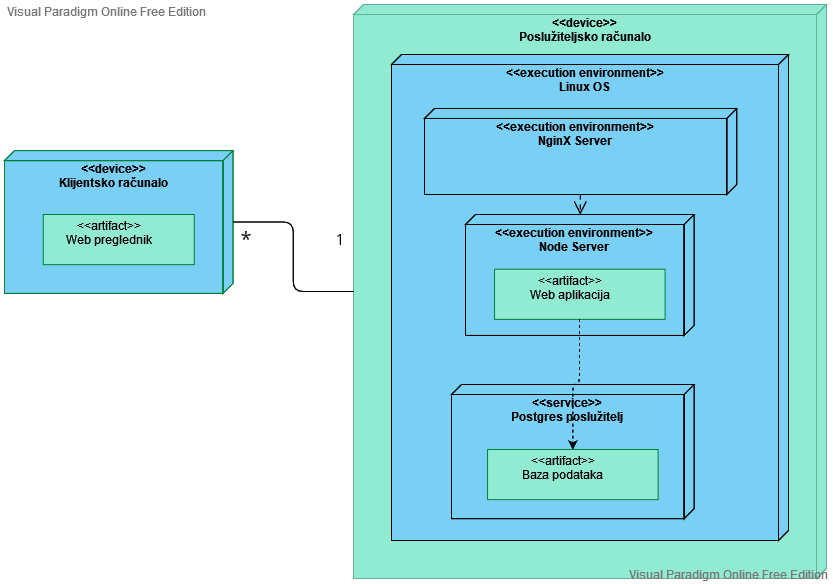
\includegraphics[width=\textwidth]{slike/dijagramrazmjestaja.png}
				\caption{Dijagram razmještaja}
				\label{fig:baza} 
			\end{figure}
			
			\eject 
		
		\section{Upute za puštanje u pogon}
			\subsection{Lokalno pokretanje}
				Da bi se cijela aplikacija pokrenula trebate imati pristup nekoj postgres bazi 
				podataka (može biti lokalno ili udaljeno/docker). Da biste instalirali pakete 
				preporučuje se yarn ali može i s npm-om, pokrenite yarn ili npm install u folderima 
				frontend i backend. Nakon toga ako želite pokrenuti backend, u backend folderu 
				trebate kopirati .env.example u .env i popuniti ga s podatcima za pristup vašoj 
				bazi podataka. Nakon toga trebate pokrenuti yarn db:rebuild sto će pokrenuti sve 
				migracije te ubaciti osnovne podatke u bazu. 
				Nakon toga prelazimo na frontend, njega možete pokrenuti i bez backenda 
				(spajajući se na produkcijski backend). Nakon sto ste pokrenuli yarn trebate kopirati 
				.env.example u .env i dodati token od vašeg MapBox računa. Za spajanje na udaljeni 
				backend možete zamijeniti localhost u NEXT\_PUBLIC\_APOLLO\_SERVER s udaljenim linkom. 
				To je sve što vam treba od postavljanja.
				Za pokretanje backenda lokalno koristite yarn dev, dok za frontend 
				koristite yarn dev i ako želite automatski generirati graphql queryje yarn gen:watch, 
				no njih možete i manualno pokretati s yarn gen svaki puta kada napravite promjenu
			
			\subsection{Puštanje u pogon na udaljenom serveru}
			Mi smo za ovo koristili linux VPS server tvrtke Vultr na kojemu je bio instaliran Ubuntu. Za samo pokretanje koristili smo node alat pm2. Na serveru smo klonirali repository, pokrenuli yarn u oba foldera te nakon toga pokrenuli yarn frontend:build unutar backenda, to izgenerira produkcijsku verziju frontenda. Nakon toga smo sa pm2 startOrRestart ecosystem.config.js u rootu projekta pokrenuli serveri cijele aplikacije

			Dodatno smo setupirali i nginx da bi dobili reverse proxy za domenu, te bazu podataka na istom serveru (ali to ovisi od servera do servera, pa nećemo ici u detalje)
			
			\eject 